\documentclass{beamer}

\usepackage[USenglish]{babel}
\usepackage[backend=bibtex,citestyle=authortitle]{biblatex}
\usepackage[scale=2]{ccicons}
\usepackage{graphicx}
\usepackage{listings}
\usepackage{tikz}

% this actually isn't totally hideous:
\usetheme[numbering=counter, progressbar=frametitle, sectionpage=none]{metropolis}

\graphicspath{{../figures/}}

\title{Composable Concurrency Models}
\date{November 19, 2016}
\author{Dan Stelljes}

\bibliography{references}

\begin{document}
  \maketitle

  \section{Introduction}

  \begin{frame}
    \begin{figure}
      \begin{tikzpicture}
        \onslide<1->{
          \node at (0,0) {
            
\includegraphics[width=300pt]{browser}
          };
        }

        \onslide<2>{
          \path (-2.25,2.75) [draw=none, fill=darkgray, opacity=0.75] ellipse (60pt and 25pt);
          \node [text=white] at (-2.25,2.75) {
            Multiple tabs
          };

          \draw (2.25,2.25) [draw=none, fill=darkgray, opacity=0.75] ellipse (60pt and 25pt);
          \node [text=white] at (2.25,2.25) {
            Suggestions
          };

          \draw (0,0.5) [draw=none, fill=darkgray, opacity=0.75] ellipse (60pt and 25pt);
          \node [text=white] at (0,0.5) {
            Page rendering
          };

          \draw (-3,-1.5) [draw=none, fill=darkgray, opacity=0.75] ellipse (60pt and 25pt);
          \node [text=white] at (-3,-1.5) {
            Event handling
          };

          \draw (2.5,-1.5) [draw=none, fill=darkgray, opacity=0.75] ellipse (60pt and 25pt);
          \node [text=white] at (2.5,-1.5) {
            Background processes
          };
        }

        \onslide<3>{
          \node at (0,-0.62) {
            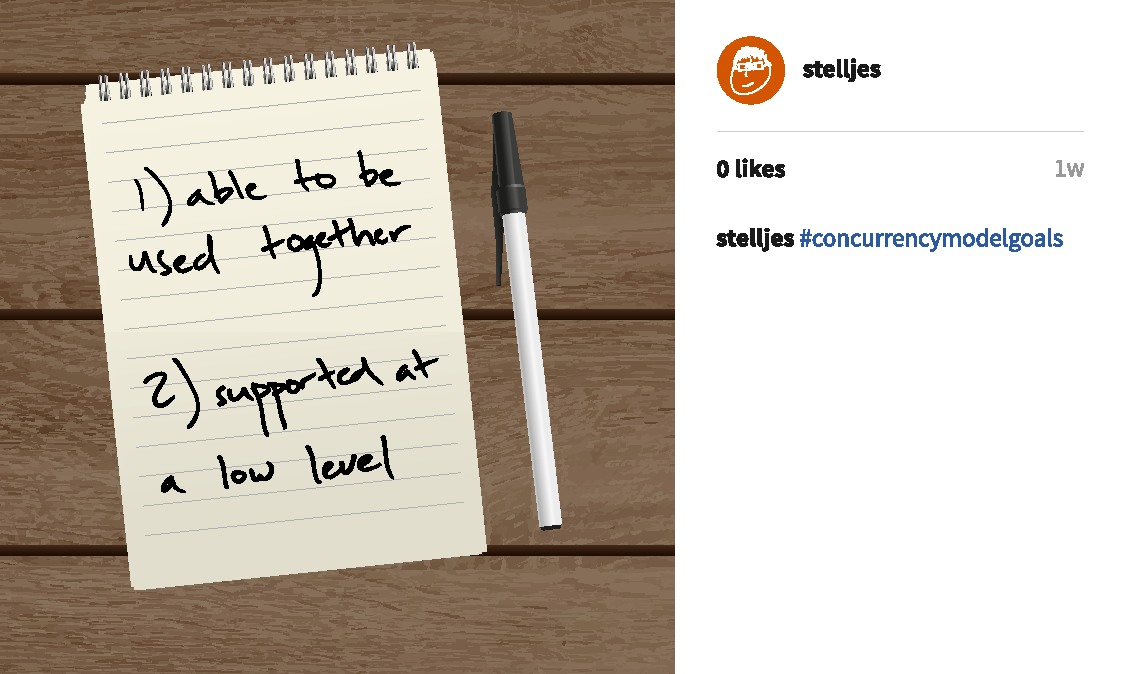
\includegraphics[width=220pt]{goals}
          };
        }
      \end{tikzpicture}
    \end{figure}
  \end{frame}

  \section{Background}

  \subsection{Concurrency}

  \begin{frame}
    \frametitle{Concurrency}
    \framesubtitle{Intuitive definition}

    \onslide<1>{
      \begin{columns}[T]
        \begin{column}{0.48\textwidth}
          \centering
          sequential
        \end{column}

        \hfill

        \begin{column}{0.48\textwidth}
          \centering
          concurrent
        \end{column}
      \end{columns}
    }

    \onslide<2>{
      \begin{columns}[T]
        \begin{column}{0.48\textwidth}
          \centering
          concurrent
        \end{column}

        \hfill

        \begin{column}{0.48\textwidth}
          \centering
          parallel
        \end{column}
      \end{columns}
    }
  \end{frame}

  \begin{frame}
    \frametitle{Concurrency}
    \framesubtitle{Formal definition}

    \textbf{The ``happens before'' ($\rightarrow$) relation~\footcite{Lamport1977}}

    $A \rightarrow B$ if one of the following is true:

    \begin{enumerate}
      \item $A$ and $B$ are operations in the same thread and $A$ occurs before $B$.
      \item $A$ is the sending of a message by one thread and $B$ is the receipt of the same message by another thread.
    \end{enumerate}

    $A$ and $B$ are said to be concurrent if $A \nrightarrow B$ and $B \nrightarrow A$.
  \end{frame}

  \subsection{Consistency}

  \begin{frame}
    \frametitle{Consistency models}

    \begin{itemize}
      \item \textbf{Sequential:} Does the history of the program yield a correct result?
      \item \textbf{Concurrent:} Does every possible history of the program yield a correct result?
    \end{itemize}
  \end{frame}

  \begin{frame}
    \frametitle{Complications}

    \onslide<1->{
      \centering
      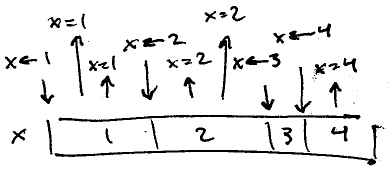
\includegraphics{single-thread-read-write}
    }

    \onslide<2->{
      \centering
      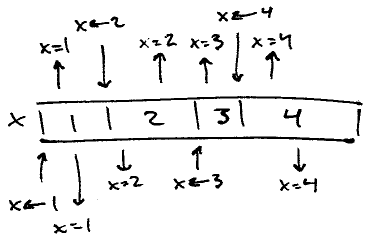
\includegraphics{multiple-threads-read-write}
    }
  \end{frame}

  \begin{frame}
    \frametitle{Complications}

    \begin{figure}
      \centering
      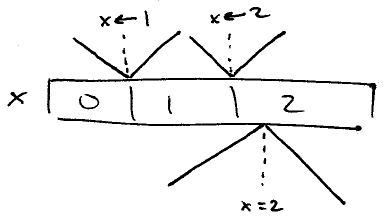
\includegraphics{noninstantaneity}
    \end{figure}
  \end{frame}

  \subsection{Correctness}

  \begin{frame}
    \frametitle{Linearizability}

    \begin{figure}
      \centering
      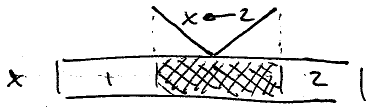
\includegraphics{linearizability}
    \end{figure}

    \begin{itemize}
      \item Linearizability guarantees that the completion of an operation on a single object will appear to be instantaneous.
      \item The results of a linearizable operation will be visible as soon as the operation is complete.
    \end{itemize}
  \end{frame}

  \begin{frame}
    \frametitle{Serializability}

    \begin{figure}
      \centering
      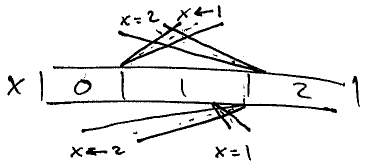
\includegraphics{serializability}
    \end{figure}

    \begin{itemize}
      \item Serializability guarantees that operations can occur in any order as long as an equivalent serial history exists.
      \item While a serializable set of operations is being executed, it appears to be the only set of operations being executed.
    \end{itemize}
  \end{frame}

  \begin{frame}
    \frametitle{Strict serializability}

    \begin{itemize}
      \item Linearizability is a guarantee of consistency.
      \item Serializability is a guarantee of isolation.
      \item Together, linearizability and serializability guarantee strict serializability---a history is equivalent to some serial execution order and that order corresponds to the execution order in real time.
    \end{itemize}
  \end{frame}

  \section{Common concurrency models}

  \begin{frame}
    \frametitle{Concurrency models}

    \begin{itemize}
      \item Modern languages usually support several different models.
      \item Common concurrency models can be generalized:~\footcite{Swalens2014}
      \begin{enumerate}
        \item Atomic variables
        \item Software transactional memory (STM)
        \item Communicating threads
        \item Proxies
      \end{enumerate}
    \end{itemize}
  \end{frame}

  \subsection{Atomic variables}

  \begin{frame}[fragile]
    \frametitle{Atomic variables}

    \begin{itemize}
      \item Atomic variables can only be read and mutated by linearizable operations:
    \end{itemize}

    \begin{lstlisting}[basicstyle=\scriptsize\ttfamily,language=C]
      bool compare_and_swap(int* v, int old, int new) {
        if (*v != old) {
          return false;
        }

        *v = new;
        return true;
      }
    \end{lstlisting}

% "good indentation? lol get bent" —Beamer
\end{frame}

  \subsection{Software transactional memory}

  \begin{frame}
  \end{frame}

  \subsection{Communicating threads}

  \begin{frame}
  \end{frame}

  \subsection{Proxies}

  \begin{frame}
  \end{frame}

  \section{Composability challenges}

  \subsection{Possible conflicts}

  \section{Proposed abstractions}

  \subsection{Ownership-based meta-object protocol}

  \section{Conclusion}

  \begin{frame}
    \frametitle{Future work}
  \end{frame}

  \begin{frame}[standout]
    \centering

    \url{github.com/dstelljes/senior-sem}

    \vfill

    \ccbyncsa{}
  \end{frame}

\end{document}
